\subsection{Context}
The current engineering prowesses allow us to construct buildings higher and higher. These constructions are subject to various disturbances (mainly wind, but also earthquakes) that make them oscillate. They turn into giant pendulum and swing from left to right, sometimes moving several meters at the top !\cite{YouTube_minutephysics}\par
To reduce these oscillations, we use a passive system, called {\it tuned mass damper}, which consists of concealing a tuned and harmonic oscillator at the top of the tower. It is coupled to its movement and oscillates in phase opposition to recover the kinetic energy of the tower and thus reduces the oscillations.\cite{Wikipedia_amortisseur_tmd}\par
An active version of this system exists : the {\it active mass damper}. It consists of the same principle as the tuned mass damper but it is equipped with sensors and actuators to measure the oscillations of its environment and, via an algorithm, generate a movement for the mass that reduce, or totally remove, these oscillations.\cite{sciencedirect_amd}\par
Our study field focuses on the active mass damper systems used to reduce the oscillations caused by the {\bf wind} on {\bf tall} buildings. More specifically, we will focus on a simplified model : a block linked to a spring (to simulate the oscillations of the building) and a smaller moving mass placed over it that stabilises the system.\par
This model is presented in figure \ref{fig:schema}.
\begin{figure}[!ht]
    \centering
    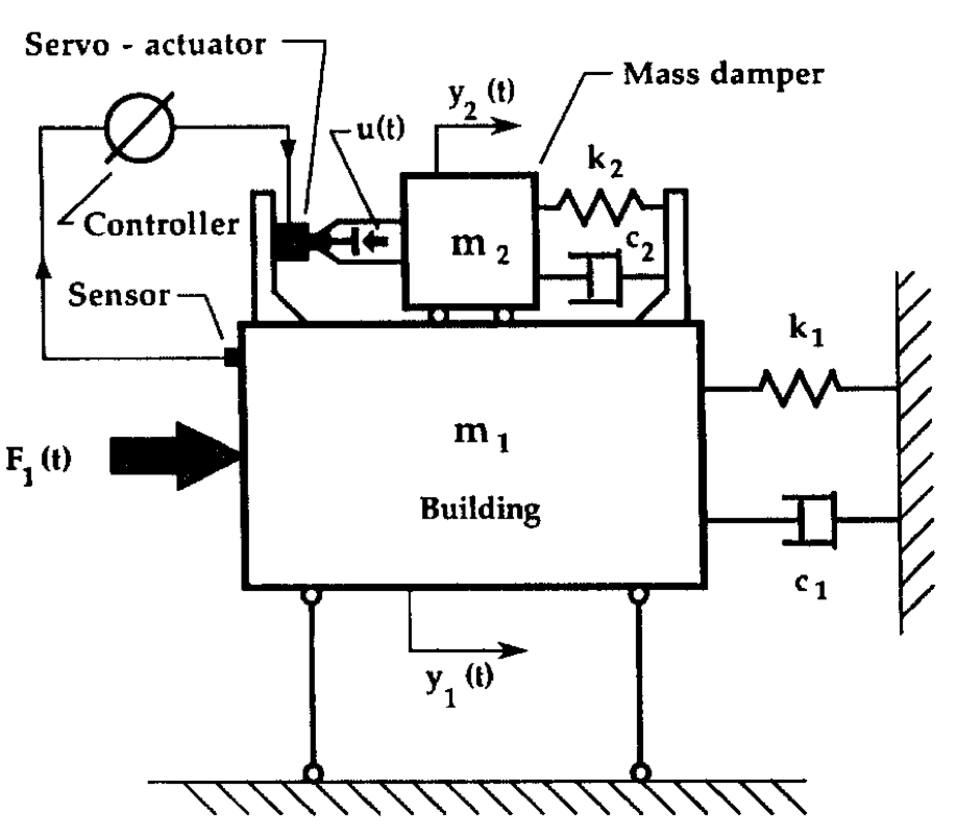
\includegraphics[width=0.7\textwidth]{resources/pdf/schema.pdf}
    \caption{Model of an active mass damper for the stabilization of a tall building \cite{sciencedirect_amd_2}}
    \label{fig:schema}
\end{figure}
